\documentclass[11pt,a4paper]{article}

\usepackage[T1]{fontenc}
\usepackage[utf8]{inputenc}
\usepackage[margin=2.4cm]{geometry}
\usepackage{amsmath,amssymb,amsthm,mathtools}
\usepackage{xcolor}
\usepackage{booktabs,array,enumitem}
\usepackage{float}
\usepackage[most]{tcolorbox}
\usepackage{tikz}
\usetikzlibrary{arrows.meta,positioning,calc,shapes.geometric,decorations.pathreplacing,fit,backgrounds}
\usepackage{pgfplots}
\pgfplotsset{compat=1.16}
\emergencystretch=2em
\usepackage[colorlinks=true,linkcolor=blue!50!black,urlcolor=blue!50!black]{hyperref}

% ---------- macros ----------
\newcommand{\E}{\mathbb{E}}
\newcommand{\PP}{\mathbb{P}}
\newcommand{\cS}{\mathcal{S}}
\newcommand{\cA}{\mathcal{A}}
\newcommand{\Rmax}{R_{\max}}
\DeclareMathOperator*{\argmax}{arg\,max}
\newcommand{\slr}[1]{\texorpdfstring{\emph{(slides #1)}}{(slides #1)}}

% ---------- theorem-like environments (amsthm, boxed) ----------
\theoremstyle{plain}
\newtheorem{theorem}{Theorem}[section]
\newtheorem{lemma}[theorem]{Lemma}
\newtheorem{proposition}[theorem]{Proposition}
\newtheorem{corollary}[theorem]{Corollary}
\theoremstyle{definition}
\newtheorem{definition}[theorem]{Definition}
\newtheorem{example}[theorem]{Example}
\newtheorem{algorithm}[theorem]{Algorithm}
\theoremstyle{remark}
\newtheorem*{remark}{Remark}

\tcbset{thmbox/.style={breakable,colback=black!3,colframe=black!55,boxrule=0.5pt,arc=1.5mm,
  left=3mm,right=3mm,top=1mm,bottom=1mm,before skip=9pt,after skip=9pt}}
\tcolorboxenvironment{theorem}{thmbox}
\tcolorboxenvironment{lemma}{thmbox}
\tcolorboxenvironment{proposition}{thmbox}
\tcolorboxenvironment{corollary}{thmbox}
\tcolorboxenvironment{definition}{thmbox}
\tcolorboxenvironment{example}{thmbox}
\tcolorboxenvironment{algorithm}{thmbox}

% ---------- blue Intuition box ----------
\newtcolorbox{intuition}{enhanced,breakable,colback=blue!4!white,colframe=blue!55!black,
  coltitle=white,colbacktitle=blue!55!black,title={Intuition},fonttitle=\bfseries\small,
  boxrule=0.6pt,arc=1.5mm,left=3mm,right=3mm,top=1.5mm,bottom=1.5mm,before skip=8pt,after skip=11pt}

% ---------- placeholder for figures that must be taken from the slides ----------
\newcommand{\slideplaceholder}[3][3.6cm]{%
  \begin{center}\begin{tikzpicture}
  \node[draw=gray,dashed,thick,fill=gray!6,minimum width=0.82\linewidth,minimum height=#1,
        align=center,text=gray!60!black,text width=0.74\linewidth]
        {\textbf{[Insert figure from slide #2]}\\[2pt]\small #3};
  \end{tikzpicture}\end{center}}

\title{\textbf{Lecture 3 --- Markov Decision Processes}\\[2pt]
\large Reinforcement Learning 2026--27 \\[-1pt] \normalsize (slides by Roberto Capobianco; companion text: book chapter 4)}
\author{Lecture notes}
\date{}

\begin{document}
\maketitle
\begin{center}\small
Structure follows the slide deck (slides 1--55); formal statements and proofs are merged in from the
companion PDF at the point where the slides introduce the topic. Material that appears only in the PDF is
collected in the Appendix.
\end{center}
\tableofcontents
\bigskip

%=====================================================================
\section{Recap \slr{2--11}}
%=====================================================================
The lecture opens by recalling the bandit material of the previous lectures (slide 2 opens the recap, slide 11 closes it). The point of the recap is to set up the jump from \emph{one-step} decision making to \emph{sequential} decision making.

\subsection{From Multi-Armed to Contextual Bandits \slr{3}}
A multi-armed bandit (MAB) is stateless: the agent picks an action and receives a reward. A \emph{contextual bandit} (CB) adds back some context (a state): before acting, the agent sees a context $x_t$, and the reward depends on both the context and the arm.

\begin{figure}[htbp]
\centering
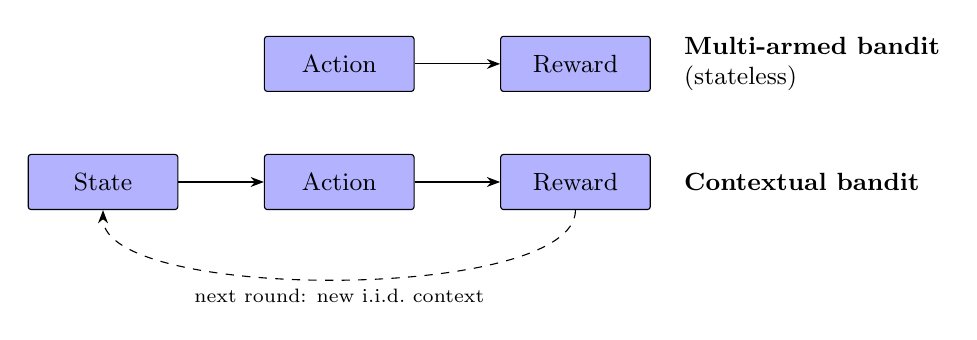
\begin{tikzpicture}[>=Stealth,
  box/.style={draw,fill=blue!30,rounded corners=1pt,minimum width=1.9cm,minimum height=0.7cm,font=\small}]
  \node[box] (a1) at (0,1.5) {Action};
  \node[box] (r1) at (3,1.5) {Reward};
  \draw[->] (a1)--(r1);
  \node[anchor=west,align=left,font=\small] at ([xshift=3mm]r1.east) {\textbf{Multi-armed bandit}\\(stateless)};
  \node[box] (s2) at (-3,0) {State};
  \node[box] (a2) at (0,0) {Action};
  \node[box] (r2) at (3,0) {Reward};
  \draw[->] (s2)--(a2); \draw[->] (a2)--(r2);
  \node[anchor=west,align=left,font=\small] at ([xshift=3mm]r2.east) {\textbf{Contextual bandit}};
  \draw[->,dashed] (r2.south) to[out=-90,in=-90,looseness=0.5]
     node[below,font=\scriptsize]{next round: new i.i.d.\ context} (s2.south);
\end{tikzpicture}
\caption{MAB versus contextual bandit (redrawn from slide 3).}
\end{figure}

\begin{intuition}
Think of a MAB as a single slot machine room with no information about who walks in; a CB is the same room where each customer has a profile $x_t$ and the best machine depends on the profile. The crucial point for what follows: in a CB the context is drawn i.i.d., so \emph{my action does not change the next context}. MDPs remove exactly this restriction.
\end{intuition}

\subsection{Contextual Bandits: Interaction \slr{4}}
For $t=0,\dots,T-1$:
\begin{enumerate}[nosep]
  \item a new i.i.d.\ context $x_t\in\mathcal X$ appears;
  \item select an action $a_t\in\cA$ based on historical information and the context;
  \item observe the reward $r(x_t,a_t)$ (context- and arm-dependent).
\end{enumerate}
For simplicity the rewards are assumed deterministic, ``as the context is the challenge here''.

\subsection{Contextual Bandits: Regret \slr{5}}
The optimal policy is $\pi^\star=\argmax_{\pi\in\Pi}\E_{x\sim\mu}[r(x,\pi(x))]$. At every iteration $a_t=\pi^t(x_t)$ is chosen, and the regret compares the total expected reward of always using $\pi^\star$ with that of our learned sequence of policies:
\[
  \mathrm{Regret}_T \;=\; T\,\E_{x\sim\mu}\!\left[r(x,\pi^\star(x))\right]\;-\;\sum_{t=0}^{T-1}\E_{x\sim\mu}\!\left[r(x,\pi^t(x))\right].
\]
Note that the policies $\pi^t$ are different at every iteration $t$.

\begin{intuition}
Regret is ``how much reward I left on the table by not knowing $\pi^\star$ from day one''. If $\mathrm{Regret}_T$ grows sublinearly in $T$, the \emph{average} regret per round goes to $0$: eventually the learner behaves like the optimal policy.
\end{intuition}

\subsection{Explore \& Commit Algorithm \slr{6}}
\begin{algorithm}[Explore \& Commit for contextual bandits]
\begin{enumerate}[nosep]
  \item For $t=0,\dots,N-1$ (\emph{explore}): observe $x_t\sim\mu$; sample $a_t\sim\mathrm{Unif}(\cA)$; observe $r_t=r(x_t,a_t)$; build, for $x_t$, an unbiased estimate $\hat r_t$ of the reward vector, with $\E_{a_t\sim\mathrm{Unif}(\cA)}\hat r_t[a]=r(x_t,a)\ \forall a$:
  \[
   \hat r_t[a]=\begin{cases}0 & a\neq a_t\\[2pt] \dfrac{r_t}{1/|\cA|} & a=a_t.\end{cases}
  \]
  \item Compute the policy $\hat\pi=\argmax_{\pi\in\Pi}\sum_{t=0}^{N-1}\hat r_t[\pi(x_t)]$.
  \item For $t=N,\dots,T-1$ (\emph{commit}): observe $x_t\sim\mu$ and play $a_t=\hat\pi(x_t)$.
\end{enumerate}
\end{algorithm}
With a suitable $N$ the regret is
\[
  \mathrm{Regret}_T=O\!\left(T^{2/3}K^{1/3}\ln(|\Pi|)^{1/3}\right),\qquad K=|\cA|.
\]

\begin{intuition}
The division by $1/|\cA|$ is \emph{importance weighting}: we only see the reward of the arm we actually played, which happens with probability $1/|\cA|$, so we inflate it by $|\cA|$ to be right on average. A numerical feel for the rate: doubling the horizon multiplies the regret bound by only $2^{2/3}\approx1.59$, so the per-round regret decays like $T^{-1/3}$.
\end{intuition}

\subsection{\texorpdfstring{$\epsilon$}{epsilon}-Greedy \slr{7}}
Instead of fixing a threshold for exploring and then committing, interleave exploration and exploitation. For $t=0,\dots,T$: observe $x_t\sim\mu$; draw
\[
  a_t\sim p_t=(1-\epsilon)\,\delta\big(\pi^t(x_t)\big)+\epsilon\,\mathrm{Unif}(\cA);
\]
observe $r_t=r(x_t,a_t)$; build an unbiased estimate $\hat r_t$ for $x_t$ (so that $\E_{a\sim p_t}\hat r_t[a]=r(x_t,a)$); update the policy $\pi^{t+1}=\argmax_{\pi\in\Pi}\sum_{\tau\le t}\hat r_\tau[\pi(x_\tau)]$. Here $\epsilon=0$ means pure exploitation and $\epsilon=1$ uniform exploration. (The slide only asserts unbiasedness; the usual choice is the importance-weighted estimator $\hat r_t[a]=\mathbb 1[a=a_t]\,r_t/p_t(a_t)$.)

\begin{intuition}
Explore \& Commit explores first, then stops learning. $\epsilon$-greedy never stops: with $\epsilon=0.1$, about one round in ten is a random experiment, and the other nine use the current best guess. It is robust to the case where the early estimates were wrong.
\end{intuition}

\subsection{Bayesian Bandits \slr{8}}
So far no assumption was made about the reward distributions $\nu_i$; only bounds on rewards were derived. In Bayesian bandits we (i) exploit \emph{prior} knowledge of rewards, (ii) update a \emph{posterior} distribution from historical information, and (iii) use the posterior to guide exploration, either through upper confidence bounds (Bayesian UCB) or probability matching (Thompson sampling).

\subsection{Gaussian Bayesian Bandits: UCB \slr{9}}
Now that a distribution is modelled, a notion of confidence comes for free: for Gaussians it is the standard deviation. The UCB rule picks
\[
  a_t=\argmax_{i\in K}\;\mu_t(i)+\frac{c\,\sigma_t(i)}{\sqrt{N_t(i)}},
\]
where $N_t(i)$ is the number of pulls of arm $i$ and $c$ a constant.

\subsection{Gaussian Bayesian Bandits: Thompson Sampling \slr{10}}
For $t=0,\dots,T$: for each arm $i=1,\dots,K$ sample $\tilde r_t(i)$ independently from $\mathcal N(\mu_{t-1}(i),\sigma^2_{t-1}(i))$; pull $I_t=\argmax_i\tilde r_t(i)$; observe $r_t$; update the posterior $p(\mu_t(i),\sigma_t^2(i)\mid r_t)$. This can be done with other distributions as well. The slide stresses that this is an estimate of the \emph{reward}: in more general MDPs it is replaced by the $Q$ function, i.e.\ we estimate a distribution over $Q$.

\begin{figure}[htbp]
\centering
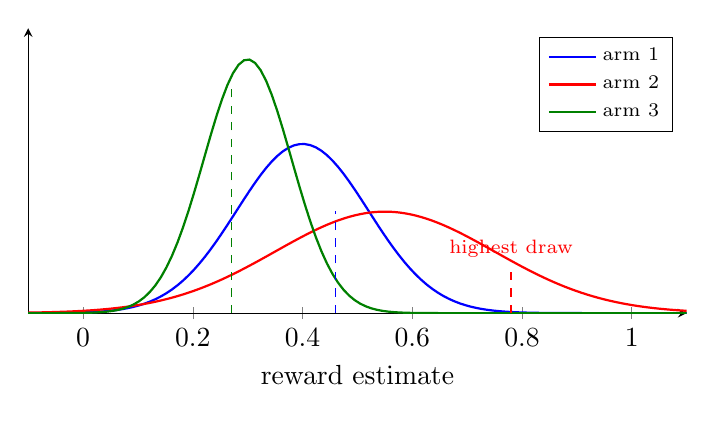
\begin{tikzpicture}
\begin{axis}[width=0.82\linewidth,height=5.2cm,xlabel={reward estimate},ytick=\empty,
  axis lines=left,legend style={font=\scriptsize,at={(0.98,0.97)},anchor=north east},
  domain=-0.1:1.1,samples=120,ymin=0,ymax=5.6]
 \addplot[blue,thick]{exp(-0.5*((x-0.40)/0.12)^2)/(0.12*2.5066)};
 \addplot[red,thick]{exp(-0.5*((x-0.55)/0.20)^2)/(0.20*2.5066)};
 \addplot[green!50!black,thick]{exp(-0.5*((x-0.30)/0.08)^2)/(0.08*2.5066)};
 \legend{arm 1,arm 2,arm 3}
 \addplot[blue,dashed] coordinates{(0.46,0)(0.46,2.0)};
 \addplot[red,dashed] coordinates{(0.78,0)(0.78,0.8)};
 \addplot[green!50!black,dashed] coordinates{(0.27,0)(0.27,4.5)};
 \node[red,font=\scriptsize,anchor=south] at (axis cs:0.78,0.9) {highest draw};
\end{axis}
\end{tikzpicture}
\caption{Thompson sampling with Gaussian posteriors (original illustration of the idea on slide 10; the numbers are illustrative). Dashed lines are the independent draws $\tilde r(i)$; the uncertain arm~2 gets the highest draw and is pulled.}
\end{figure}

\begin{intuition}
Thompson sampling explores in proportion to uncertainty without any explicit exploration parameter: an arm with a wide posterior occasionally produces a high draw and gets tried; once its posterior narrows and its mean is low, the draws stop beating the others. This is the ``probability matching'' idea: pull each arm with the probability that it is the best.
\end{intuition}

%=====================================================================
\section{Sequential Decision Making \slr{12--14}}
%=====================================================================
The agent interacts with the environment at discrete time steps, by receiving an observation $o_t$ and a reward $r_t$ from the environment and by taking actions $a_t$ (slide 12).

\begin{figure}[htbp]
\centering
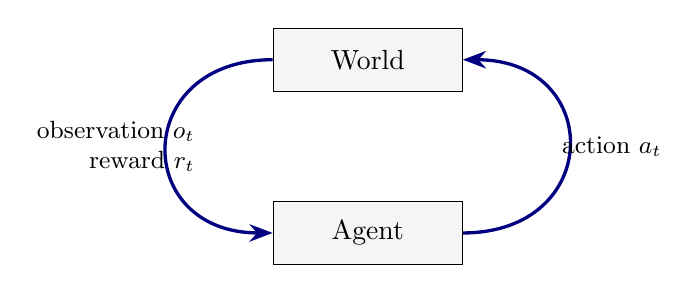
\begin{tikzpicture}[>=Stealth,
  box/.style={draw,minimum width=2.4cm,minimum height=0.8cm,fill=gray!8}]
  \node[box] (w) at (0,2.2) {World};
  \node[box] (ag) at (0,0) {Agent};
  \draw[->,very thick,blue!50!black] (w.west) .. controls (-3,2.2) and (-3,0) .. (ag.west);
  \draw[->,very thick,blue!50!black] (ag.east) .. controls (3,0) and (3,2.2) .. (w.east);
  \node[align=right,font=\small] at (-3.2,1.1) {observation $o_t$\\ reward $r_t$};
  \node[font=\small] at (3.1,1.1) {action $a_t$};
\end{tikzpicture}
\caption{The agent--world loop (slides 12--14, redrawn).}
\end{figure}

Such a discrete interaction generates a trajectory, or \emph{history}, at each time step $t$, which the agent uses to choose its action (slide 13):
\[
  h_t=(o_0,a_0,r_1,o_1,a_1,\dots,r_t,o_t,a_t)\quad\text{(indexing convention as on the slide)}.
\]
The \emph{state} is a function of the history, $s_t=f(h_t)$, and it is typically hidden or unknown (slide 14).

\begin{intuition}
The history grows without bound; no practical agent can condition on all of it. The state is a \emph{summary} of the history that is supposed to keep what matters for the future. Which summary is a good one is exactly the question the Markov assumption answers.
\end{intuition}

%=====================================================================
\section{Markov Assumption \slr{15--17}}
%=====================================================================
\begin{definition}[Markov state]\label{def:markov}
A state representation is Markov if for every $t$, every history $h_t$ and every action $a_t$,
\[
  p(s_{t+1}\mid s_t,a_t)=p(s_{t+1}\mid h_t,a_t).
\]
The future is conditionally independent of the past given the present.
\end{definition}

\begin{intuition}
If I tell you the current state and my action, nothing in the earlier history can sharpen your prediction of the next state. A chess position is Markov (how we reached it is irrelevant for what can happen next). The position of a moving ball alone is \emph{not}: without its velocity, the past positions carry extra information.
\end{intuition}

\begin{figure}[H]
	\centering
	
\includegraphics[width=1.0\linewidth]{1790936412217.png}
	\caption{Is this problem Markovian?}\label{fig:1790936412217}
\end{figure}
Slide 16 asks, over a picture of a robot in a corridor with two pillars, ``Is this problem Markovian?'' The answer depends on what we put in the state: if the state is only the robot's position but the dynamics depend on, e.g., its velocity or an unobserved internal variable, past observations help predict the future and the state is \emph{not} Markov; adding the missing variables restores the property.


Slide 17 gives the two extremes:
\begin{itemize}[nosep]
  \item a state can \emph{always} be made Markov by taking it equal to the whole history, $s_t=h_t$;
  \item the best case, used in practice, is that the state is (a sufficient statistic of) the latest observation, $s_t=o_t$. The state is then said to be \emph{fully observable}.
\end{itemize}

\begin{figure}[htbp]
\centering
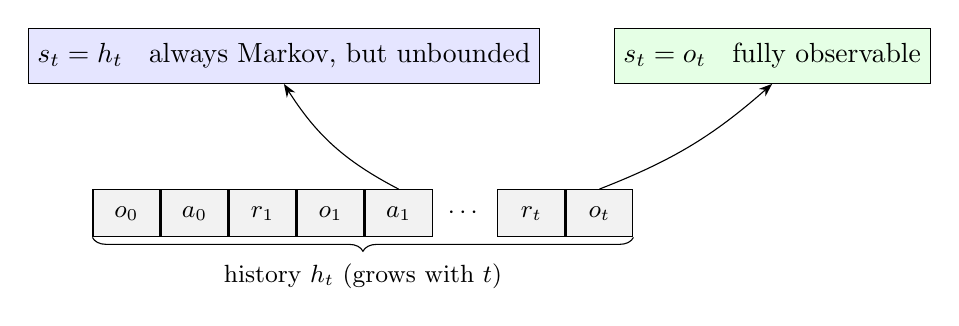
\begin{tikzpicture}[>=Stealth,
  it/.style={draw,minimum width=0.85cm,minimum height=0.6cm,font=\small,fill=gray!10}]
  \node[it](o0)at(0,0){$o_0$};\node[it,right=0pt of o0](a0){$a_0$};
  \node[it,right=0pt of a0](r1){$r_1$};\node[it,right=0pt of r1](o1){$o_1$};
  \node[it,right=0pt of o1](a1){$a_1$};\node[right=2pt of a1,font=\small](dd){$\cdots$};
  \node[it,right=2pt of dd](rt){$r_t$};\node[it,right=0pt of rt](ot){$o_t$};
  \draw[decorate,decoration={brace,mirror,amplitude=5pt}] (o0.south west)--(ot.south east)
     node[midway,below=6pt,font=\small]{history $h_t$ (grows with $t$)};
  \node[draw,fill=blue!10,minimum height=0.7cm] (s1) at (2,2) {$s_t=h_t$ \; always Markov, but unbounded};
  \node[draw,fill=green!10,minimum height=0.7cm] (s2) at (8.2,2) {$s_t=o_t$ \; fully observable};
  \draw[->] (a1.north) to[bend left=15] (s1.south);
  \draw[->] (ot.north) to[bend right=10] (s2.south);
\end{tikzpicture}
\caption{Two extreme choices of state as a function of the history (original illustration of slide 17).}
\end{figure}

\begin{intuition}
Choosing $s_t=h_t$ is a cheat: it is trivially Markov, but the state space explodes with time. Practical RL wants a small state that is still Markov. Fully observable means the observation already contains everything relevant; this is the setting of the rest of the lecture.
\end{intuition}

%=====================================================================
\section{Markov Decision Process (MDP) \slr{18--19}}
%=====================================================================
An MDP is sequential decision making under the Markov assumption: Markovian transition dynamics, full observability, and a (generally) stochastic transition kernel $p(s_{t+1}\mid s_t,a_t)$. Alternative notation: $s_{t+1}\sim p(\cdot\mid s_t,a_t)$ or $s'\sim p(\cdot\mid s,a)$ (slide 19).

\begin{definition}[Markov decision process]\label{def:mdp}
A discounted infinite-horizon MDP is a tuple $(\cS,\cA,p,r,\gamma)$: a set of states, a set of actions, transition dynamics $p(s'\mid s,a)$ satisfying Definition~\ref{def:markov}, a reward function $r:\cS\times\cA\to[0,\Rmax]$, and a discount factor $\gamma\in[0,1)$. Unless stated otherwise $\cS$ and $\cA$ are finite.
\end{definition}
(The slides introduce $\gamma$ later, in the ``Infinite Horizon Discounted Setting'' part; the tuple is stated here in full for reference.)

\begin{figure}[htbp]
\centering
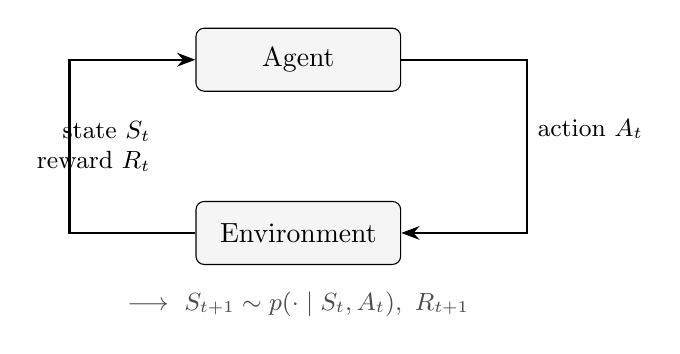
\begin{tikzpicture}[>=Stealth,
  box/.style={draw,rounded corners=3pt,minimum width=2.6cm,minimum height=0.8cm,fill=gray!8}]
  \node[box](ag) at (0,2.2){Agent};
  \node[box](en) at (0,0){Environment};
  \draw[->,thick] (ag.east) -- ++(1.6,0) |- node[pos=0.2,right,font=\small]{action $A_t$} (en.east);
  \draw[->,thick] (en.west) -- ++(-1.6,0.0) |- (ag.west);
  \node[align=right,font=\small] at (-2.6,1.1){state $S_t$\\ reward $R_t$};
  \node[font=\small,gray!60!black] at (0,-0.9){$\longrightarrow\ S_{t+1}\sim p(\cdot\mid S_t,A_t),\ R_{t+1}$};
\end{tikzpicture}
\caption{The MDP interaction loop (slides 18--19, redrawn).}
\end{figure}

\begin{intuition}
An MDP is the contextual bandit \emph{with consequences}: the next ``context'' is the next state $s'$, and it is drawn from a distribution that depends on the action just taken. Every action therefore has two effects: the reward now, and the situation in which the next decision is made.
\end{intuition}

%=====================================================================
\section{Reward \slr{20}}
%=====================================================================
A reward $r_t$ is a scalar signal representing feedback and indicating how well the agent is doing at step $t$. It is a function of state and action, written $r(s,a)$ (sometimes $r(s',a,s)$). A \emph{cost} is the negative of a reward.

\emph{Reward hypothesis} (slide 20, flagged as an open question): can all goals be achieved through the maximisation of a numerical reward?

\begin{intuition}
The reward is the only way we tell the agent what we want; everything else (what is a good state, a good action) must be \emph{derived} from it. That is why designing rewards is delicate: the agent maximises what we write, not what we meant.
\end{intuition}

%=====================================================================
\section{Deterministic MDP Example \slr{21}}
%=====================================================================
The slide shows a small deterministic MDP of a developer's day: states \emph{Wake Up} ($r=0$), \emph{Netflix} ($r=-2$, with a self-loop), \emph{Code \& Debug} ($r=-3$), \emph{Nap} ($r=1$), \emph{Deploy} ($r=10$) and \emph{Sleep} ($r=3$, terminal).

\begin{figure}[htbp]
\centering
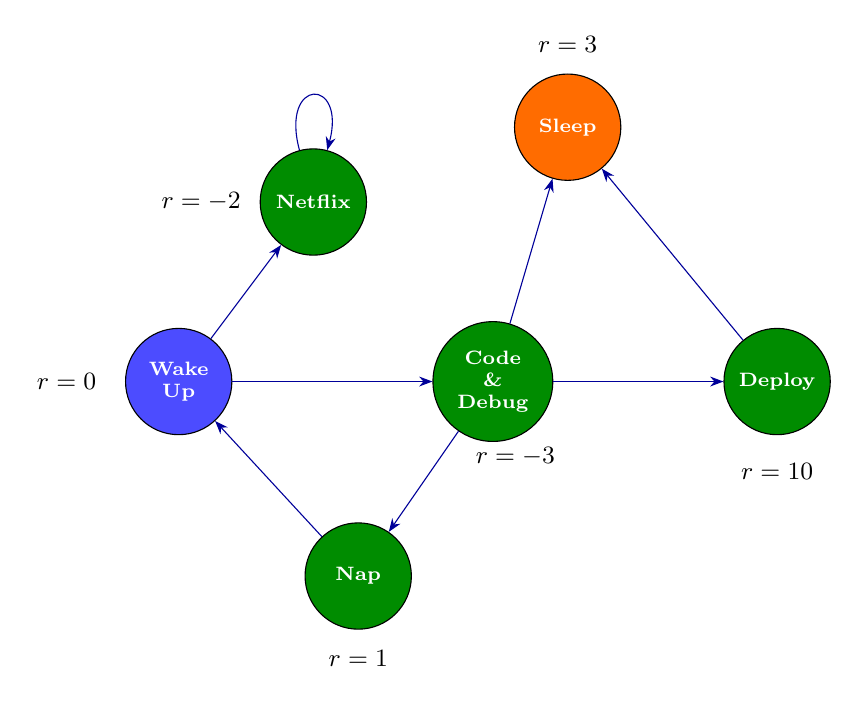
\begin{tikzpicture}[>=Stealth,scale=0.95,
  st/.style={circle,draw,minimum size=1.35cm,font=\scriptsize\bfseries,align=center,text=white,fill=green!55!black}]
  \node[st,fill=blue!70](wk) at (0,0){Wake\\Up};
  \node[st](nf) at (1.8,2.4){Netflix};
  \node[st](cd) at (4.2,0){Code\\\&\\Debug};
  \node[st,fill=orange!85!red](sl) at (5.2,3.4){Sleep};
  \node[st](dp) at (8,0){Deploy};
  \node[st](np) at (2.4,-2.6){Nap};
  \draw[->,blue!60!black] (wk)--(nf);
  \draw[->,blue!60!black] (wk)--(cd);
  \draw[->,blue!60!black] (nf) to[loop above,looseness=7] (nf);
  \draw[->,blue!60!black] (cd)--(sl);
  \draw[->,blue!60!black] (cd)--(dp);
  \draw[->,blue!60!black] (cd)--(np);
  \draw[->,blue!60!black] (np)--(wk);
  \draw[->,blue!60!black] (dp)--(sl);
  \node[font=\small] at (-1.5,0){$r=0$};
  \node[font=\small] at (0.3,2.4){$r=-2$};
  \node[font=\small] at (4.5,-1.0){$r=-3$};
  \node[font=\small] at (5.2,4.5){$r=3$};
  \node[font=\small] at (8,-1.2){$r=10$};
  \node[font=\small] at (2.4,-3.7){$r=1$};
\end{tikzpicture}
\caption{The deterministic MDP of slide 21, redrawn. Rewards are attached to states.}
\end{figure}

\begin{example}[Worked numbers, not on the slide]
Take $\gamma=0.9$, collect the reward of a state when leaving it, and treat Sleep as terminal (its reward is collected once). Then:
\begin{itemize}[nosep]
 \item $V(\text{Sleep})=3$, $V(\text{Deploy})=10+0.9\cdot3=12.7$, $V(\text{Netflix})=-2/(1-0.9)=-20$ (it can only loop).
 \item From Code \& Debug: $Q(\text{Code},\text{Deploy})=-3+0.9\cdot12.7=8.43$, $Q(\text{Code},\text{Sleep})=-3+0.9\cdot3=-0.3$. The best choice is Deploy: a ``bad'' step (reward $-3$) pays off.
 \item Hence the path Wake$\to$Code$\to$Deploy$\to$Sleep has discounted return $0+0.9\cdot8.43=7.587$, while Wake$\to$Netflix forever has return $0+0.9\cdot(-20)=-18$.
 \item Going Code$\to$Nap$\to$Wake gives $V(\text{Nap})=1+0.9\cdot7.587\approx7.83$ and $Q(\text{Code},\text{Nap})\approx4.05<8.43$, so Nap loses.
\end{itemize}
\end{example}

\begin{intuition}
The immediate reward at Code \& Debug is negative ($-3$), yet it is the right place to go through: all the value sits behind it (Deploy $=10$). A myopic agent at Wake Up compares $-2$ (Netflix) with $-3$ (Code \& Debug) and picks Netflix, where it is stuck forever with value $-20$; maximising the \emph{return} sends it through Code \& Debug instead. This is the entire reason we define value functions.
\end{intuition}

%=====================================================================
\section{Stochastic MDP Example \slr{22}}
%=====================================================================
The slide (taken from Sutton \& Barto) shows the \emph{recycling robot}: states \texttt{high} and \texttt{low} battery; actions \texttt{search}, \texttt{wait}, \texttt{recharge}. The transition table of the slide is:
\begin{center}
\renewcommand{\arraystretch}{1.15}
\begin{tabular}{llllc}
\toprule
$s$ & $a$ & $s'$ & $p(s'\mid s,a)$ & $r(s,a,s')$\\
\midrule
high & search   & high & $\alpha$   & $r_{\text{search}}$\\
high & search   & low  & $1-\alpha$ & $r_{\text{search}}$\\
low  & search   & high & $1-\beta$  & $-3$\\
low  & search   & low  & $\beta$    & $r_{\text{search}}$\\
high & wait     & high & $1$        & $r_{\text{wait}}$\\
high & wait     & low  & $0$        & --\\
low  & wait     & high & $0$        & --\\
low  & wait     & low  & $1$        & $r_{\text{wait}}$\\
low  & recharge & high & $1$        & $0$\\
low  & recharge & low  & $0$        & --\\
\bottomrule
\end{tabular}
\end{center}

\begin{figure}[htbp]
\centering
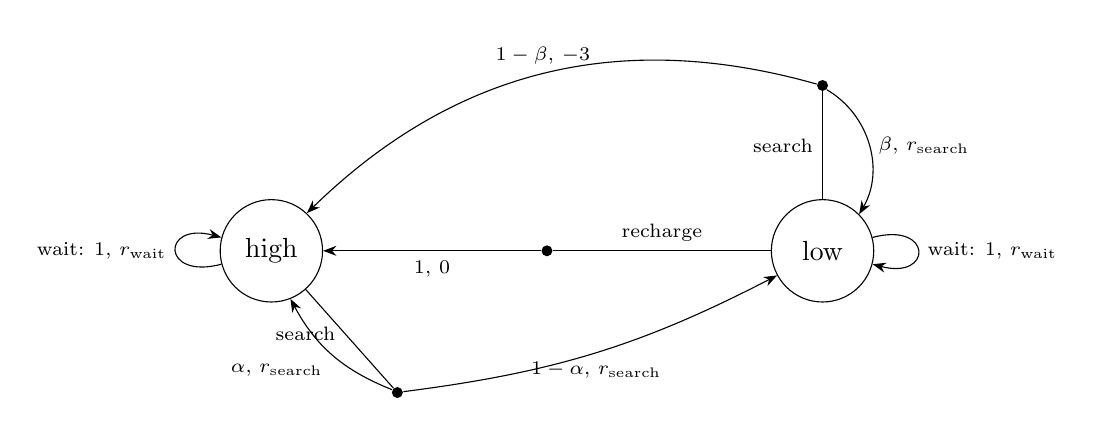
\begin{tikzpicture}[>=Stealth,
  st/.style={circle,draw,minimum size=1.3cm},
  ac/.style={circle,fill=black,inner sep=1.4pt}]
  \node[st](hi) at (0,0){high};
  \node[st](lo) at (7,0){low};
  \path (hi) edge[->,loop left,looseness=6] node[left,font=\scriptsize]{wait: $1,\,r_{\text{wait}}$} (hi);
  \path (lo) edge[->,loop right,looseness=6] node[right,font=\scriptsize]{wait: $1,\,r_{\text{wait}}$} (lo);
  % search from high
  \node[ac](sh) at (1.6,-1.8){};
  \draw (hi)--(sh) node[pos=0.45,left,font=\scriptsize]{search};
  \draw[->] (sh) to[bend left=20] node[pos=0.5,below left,font=\scriptsize]{$\alpha,\,r_{\text{search}}$} (hi);
  \draw[->] (sh) to[bend right=10] node[below,font=\scriptsize]{$1-\alpha,\,r_{\text{search}}$} (lo);
  % search from low
  \node[ac](sl) at (7,2.1){};
  \draw (lo)--(sl) node[pos=0.5,left,font=\scriptsize]{search};
  \draw[->] (sl) to[bend left=45] node[right,font=\scriptsize]{$\beta,\,r_{\text{search}}$} (lo);
  \draw[->] (sl) to[bend right=30] node[above,font=\scriptsize]{$1-\beta,\,-3$} (hi);
  % recharge
  \node[ac](rc) at (3.5,0){};
  \draw (lo)--(rc) node[pos=0.5,above,font=\scriptsize]{recharge};
  \draw[->] (rc)--(hi) node[pos=0.5,below,font=\scriptsize]{$1,\,0$};
\end{tikzpicture}
\caption{Transition graph of the recycling robot (slide 22, redrawn). Black dots are actions; edge labels are (probability, reward).}
\end{figure}

\begin{example}[Worked numbers, not on the slide]
Let $\alpha=0.7$, $\beta=0.4$, $r_{\text{search}}=2$, $r_{\text{wait}}=1$. At \texttt{low}, the expected \emph{immediate} reward of \texttt{search} is $0.4\cdot2+0.6\cdot(-3)=-1.0$, versus $+1$ for \texttt{wait}. Searching with a low battery is risky: with probability $0.6$ the robot runs flat, is rescued (reward $-3$) and ends up at \texttt{high}.
\end{example}

\begin{intuition}
Stochasticity means the same action from the same state can lead to different next states. Here a single decision (``search with a low battery'') is a gamble, and the right choice depends on the state: at \texttt{high} searching is cheap, at \texttt{low} it is not. A policy is precisely a rule for making this state-dependent choice.
\end{intuition}

%=====================================================================
\section{Policy \slr{23}}
%=====================================================================
A policy $\pi$ is a mapping from (all) states to actions that determines how the agent selects actions. It can be deterministic, $a=\pi(s)$, or stochastic, $\pi(a\mid s)$, $p(a\mid s)$ or $a\sim\pi(\cdot\mid s)$.

\begin{intuition}
A policy is a complete \emph{strategy}, not a plan: it says what to do in \emph{every} state, including the ones I might never reach. In the recycling robot there are $2\cdot3=6$ deterministic policies (two choices at \texttt{high}, three at \texttt{low}); in general there are $|\cA|^{|\cS|}$, which is why we will need structure (Bellman equations) rather than brute-force enumeration.
\end{intuition}

%=====================================================================
\section{Trajectory Probability \slr{24}}
%=====================================================================
What is the probability of seeing the trajectory $(s_0,a_0,s_1,a_1,\dots,s_t,a_t)$ at time $t$ when following $\pi$ from $s_0$? Using the Markov property and the fact that $\pi$ depends only on the current state:
\[
  \PP^\pi(s_0,a_0,\dots,s_t,a_t)=\pi(a_0\mid s_0)\,p(s_1\mid s_0,a_0)\,\pi(a_1\mid s_1)\cdots p(s_t\mid s_{t-1},a_{t-1})\,\pi(a_t\mid s_t).
\]

\begin{figure}[htbp]
\centering
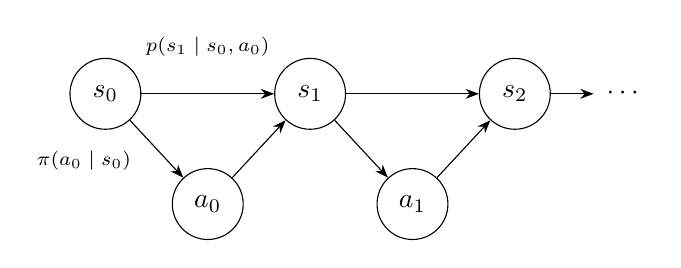
\begin{tikzpicture}[>=Stealth,
  n/.style={circle,draw,minimum size=0.9cm}]
  \node[n](s0)at(0,1.4){$s_0$};\node[n](s1)at(2.6,1.4){$s_1$};\node[n](s2)at(5.2,1.4){$s_2$};
  \node[n](a0)at(1.3,0){$a_0$};\node[n](a1)at(3.9,0){$a_1$};
  \node at (6.6,1.4){$\cdots$};
  \draw[->](s0)--(s1);\draw[->](s1)--(s2);\draw[->](s0)--(a0);\draw[->](a0)--(s1);
  \draw[->](s1)--(a1);\draw[->](a1)--(s2);\draw[->](s2)--(6.2,1.4);
  \node[font=\scriptsize] at (1.3,2.0){$p(s_1\mid s_0,a_0)$};
  \node[font=\scriptsize,anchor=east] at (0.45,0.55){$\pi(a_0\mid s_0)$};
\end{tikzpicture}
\caption{Graphical model of a trajectory (slide 24, redrawn).}
\end{figure}

\begin{intuition}
Each factor is one coin flip: the agent's flip ($\pi$) followed by the world's flip ($p$). Numbers: if $\pi(a_0|s_0)=0.5$, $p(s_1|s_0,a_0)=0.9$ and $\pi(a_1|s_1)=1$, then the probability of the length-2 trajectory $(s_0,a_0,s_1,a_1)$ is $0.5\cdot0.9\cdot1=0.45$.
\end{intuition}

%=====================================================================
\section{State Visitation Probability \slr{25--27}}
%=====================================================================
\subsection{Definition \slr{25}}
What is the probability of visiting $(s,a)$ at time $t$ when following $\pi$ from $s_0$? Marginalise the trajectory probability over everything except the last pair:
\[
  \PP^\pi_t(s,a;s_0)=\sum_{a_0,s_1,a_1,\dots,s_{t-1},a_{t-1}}\PP^\pi(s_0,a_0,\dots,s_t=s,a_t=a).
\]

\begin{intuition}
It answers ``if I run the policy many times, in what fraction of the runs am I in $(s,a)$ at time $t$?'' Plotting it for every state gives a heat map that moves and spreads with $t$.
\end{intuition}

\subsection{Examples \slr{26--27}}
Slide 26 shows, for a policy that goes to the goal in a gridworld with $10\%$ slip, the visitation probability estimated over $2000$ simulations, together with the probability mass in the (absorbing) goal as a function of $t$. Slide 27 shows the same for a \emph{random} policy, on a log scale: the mass at the goal stays essentially $0$.

\begin{figure}[htbp]
\centering
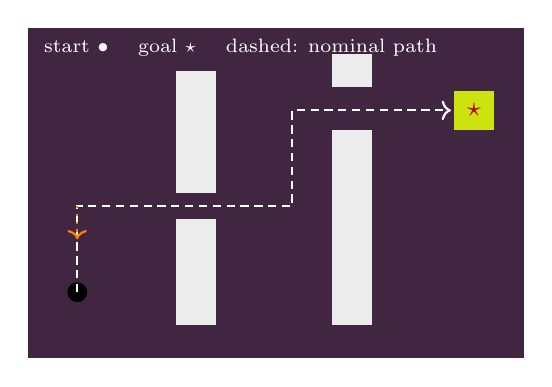
\begin{tikzpicture}[scale=0.42]
  \fill[violet!25!black!85] (0,0) rectangle (15,10);
  \fill[gray!15] (4.5,1) rectangle (5.7,4.2);
  \fill[gray!15] (4.5,5) rectangle (5.7,8.7);
  \fill[gray!15] (9.2,1) rectangle (10.4,6.9);
  \fill[gray!15] (9.2,8.2) rectangle (10.4,9.2);
  \fill[yellow!80!green] (12.9,6.9) rectangle (14.1,8.1);
  \node[red!70!black] at (13.5,7.5) {$\star$};
  \fill[black] (1.5,2) circle (0.3);
  \draw[->,thick,white,dash pattern=on 3pt off 2pt] (1.5,2)--(1.5,4.6)--(8,4.6)--(8,7.5)--(12.8,7.5);
  \draw[->,orange,dotted,thick] (1.5,4.6)--(1.5,3.6);
  \node[white,font=\scriptsize,anchor=west] at (0.2,9.4) {start $\bullet$ \quad goal $\star$ \quad dashed: nominal path};
\end{tikzpicture}
\hfill
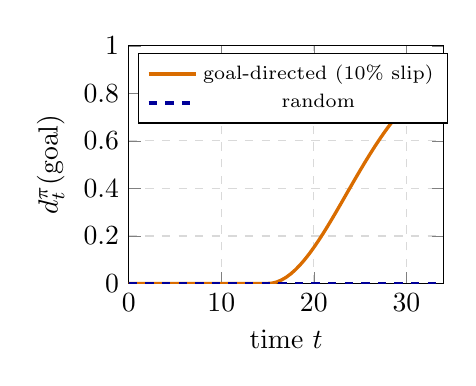
\begin{tikzpicture}
\begin{axis}[width=0.46\linewidth,height=4.6cm,xlabel={time $t$},ylabel={$d^\pi_t(\text{goal})$},
  xmin=0,xmax=34,ymin=0,ymax=1,grid=both,grid style={dashed,gray!30},domain=0:34,samples=69,
  legend style={font=\scriptsize,at={(0.03,0.97)},anchor=north west}]
 \addplot[orange!85!black,very thick]{(x>15)*0.95*(1-exp(-((x-15)/12)^2))};
 \addplot[blue!60!black,very thick,dashed]{0.0005};
 \legend{goal-directed ($10\%$ slip),random}
\end{axis}
\end{tikzpicture}
\caption{Schematic gridworld (left) and shape of the probability mass at the absorbing goal (right) for a goal-directed policy versus a random one. The curve is an original schematic read off slides 26--27, \emph{not} the data of the slide.}
\end{figure}

\begin{figure}[H]
	\centering
	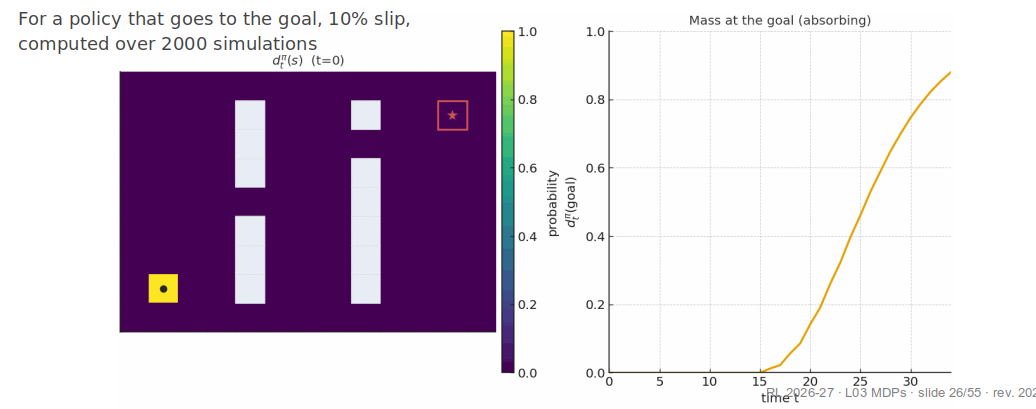
\includegraphics[width=1.0\linewidth]{1790936537236.png}
	\caption{Heat map of $d^\pi_t(s)$ for the goal-directed policy (10\% slip, 2000 simulations) with the ``mass at the goal'' curve.}\label{fig:1790936537236}
\end{figure}

\begin{figure}[H]
	\centering
	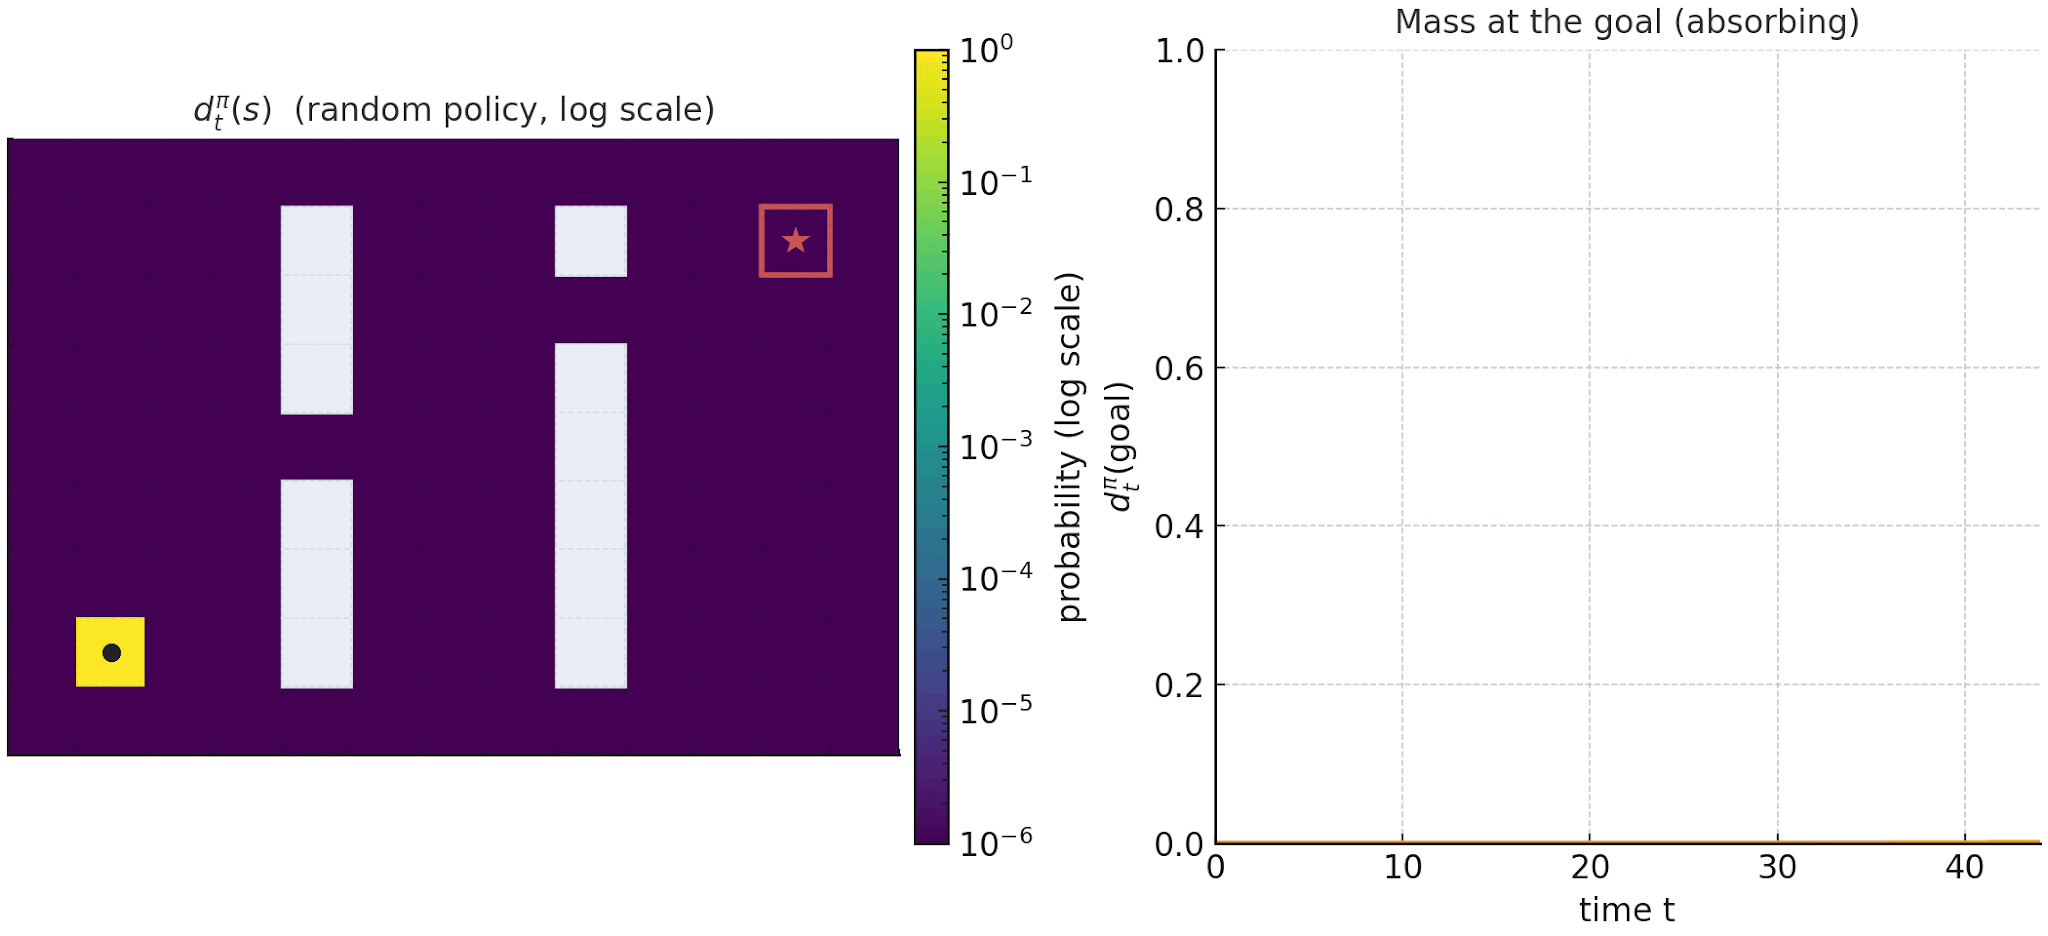
\includegraphics[width=1.0\linewidth]{1790936575533.png}
	\caption{Same for the random policy, probability on log scale.}\label{fig:1790936575533}
\end{figure}
\begin{intuition}
Under the goal-directed policy nothing reaches the goal for the first ${\sim}15$ steps (that is the minimum distance), then the mass climbs towards $1$; the missing mass is runs that slipped and are still on the way. The random policy diffuses over the grid so thinly that its goal mass is almost $0$ at every time: the visitation distribution is a fingerprint of the policy's behaviour.
\end{intuition}

%=====================================================================
\section{Another Example MDP \slr{28}}
%=====================================================================
A robotic arm that must move a ball (slide 28):
\begin{itemize}[nosep]
  \item \textbf{state:} robot configuration (joint states) and ball position;
  \item \textbf{action:} torque on arm and finger joints;
  \item \textbf{transition:} stochastic, physics plus noise;
  \item \textbf{policy:} mapping from robot state and ball position to torque;
  \item \textbf{cost:} magnitude of the torque and distance to the goal.
\end{itemize}

\begin{figure}[H]
	\centering
	
\includegraphics[width=1.0\linewidth]{1790936625953.png}
	\caption{Photo of a robotic arm manipulating a ball}\label{fig:1790936625953}
\end{figure}
\begin{intuition}
Same five ingredients, a very different world: continuous states and actions, physics instead of a table of probabilities, and a cost made of two competing terms (effort and distance to goal). The abstract tuple $(\cS,\cA,p,r)$ covers both the toy table above and a robot.
\end{intuition}

%=====================================================================
\section{Infinite Horizon Discounted Setting \slr{29}}
%=====================================================================
So far the MDP is $(\cS,\cA,p,r)$. We now add a discount factor $\gamma$ to reason about the long-term effects of a policy, with $\gamma$ in $[0,1]$ on the slide: $\gamma=0$ means ``I only care about immediate rewards'', while $\gamma=1$ means immediate and future rewards are equally important. The slide leaves ``How so?'' as a question; it is answered in ``Back to Discount Factor'' below, where we see that $\gamma=1$ is a bad idea for infinite tasks and the formal definition (Definition~\ref{def:mdp}) takes $\gamma<1$.

\begin{intuition}
$\gamma$ is a patience dial. At $\gamma=0.5$ a reward two steps away is worth $0.25$ of the same reward now; at $\gamma=0.99$ it is worth $0.98$.
\end{intuition}

%=====================================================================
\section{Value Function \slr{30--31}}
%=====================================================================
We estimate the \emph{goodness} of states and actions by their value, which is also a measure to compare policies. The state-value function of a policy $\pi$ is the expected discounted return from $s$ (slide 30):
\begin{align*}
  V^\pi(s_t)&=\E\!\left[r_t+\gamma r_{t+1}+\gamma^2r_{t+2}+\cdots\mid s_t\right]\\
  &=\E\!\left[\sum_{h=0}^{\infty}\gamma^hr_{t+h}\;\Big|\;s_t=s,\ a_h=\pi(s_h),\ s_{h+1}\sim p(\cdot\mid s_h,a_h)\right].
\end{align*}
Slide 31 adds the action-value function, where the first action is fixed and then $\pi$ is followed:
\begin{align*}
  Q^\pi(s_t,a_t)=\E\!\Big[\sum_{h=0}^{\infty}\gamma^hr_{t+h}\;\Big|\;&(s_t,a_t)=(s,a),\\
  &a_h=\pi(s_h),\ s_{h+1}\sim p(\cdot\mid s_h,a_h)\Big].
\end{align*}

\begin{intuition}
$V^\pi(s)$: ``how good is it to \emph{be} in $s$ if I then follow $\pi$?'' $Q^\pi(s,a)$: ``how good is it to take $a$ \emph{now} in $s$ and then follow $\pi$?'' The difference between the two is one free first decision. Comparing $Q^\pi(s,a)$ across $a$ is how an agent decides which action is better than the policy's current choice.
\end{intuition}

%=====================================================================
\section{Back to Discount Factor \slr{32}}
%=====================================================================
Setting $\gamma=1$ for infinite tasks is a bad idea. The quantity $\sum_{h=0}^\infty\gamma^h$ is a geometric series, equal to $1/(1-\gamma)$ for $\gamma\in[0,1)$, so the value of $\gamma$ approximately determines how many steps ahead we are looking: e.g.\ $\gamma=0.99$ corresponds to ${\sim}100$ time steps.

\begin{lemma}[Values are finite, and how finite]\label{lem:bound}
For every policy and every state, $0\le V^\pi(s)\le\dfrac{\Rmax}{1-\gamma}$.
\end{lemma}
\begin{proof}
Rewards lie in $[0,\Rmax]$, so $0\le\sum_h\gamma^hr_h\le\Rmax\sum_{h\ge0}\gamma^h=\Rmax/(1-\gamma)$, the geometric series converging because $\gamma<1$. Expectations preserve the bounds.
\end{proof}

\begin{figure}[htbp]
\centering
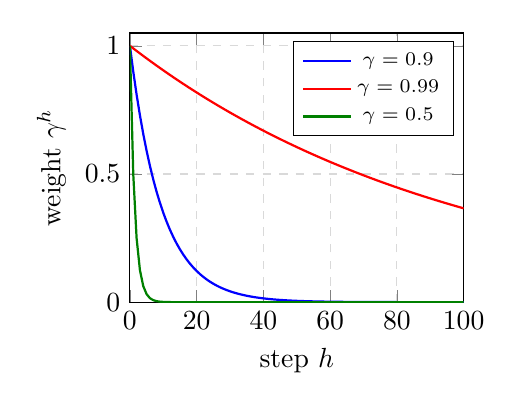
\begin{tikzpicture}
\begin{axis}[width=0.48\linewidth,height=5cm,xlabel={step $h$},ylabel={weight $\gamma^h$},xmin=0,xmax=100,ymin=0,ymax=1.05,
  legend style={font=\scriptsize,at={(0.97,0.97)},anchor=north east},domain=0:100,samples=101,grid=both,grid style={dashed,gray!30}]
 \addplot[blue,thick]{0.9^x};
 \addplot[red,thick]{0.99^x};
 \addplot[green!50!black,thick]{0.5^x};
 \legend{$\gamma=0.9$,$\gamma=0.99$,$\gamma=0.5$}
\end{axis}
\end{tikzpicture}
\hfill
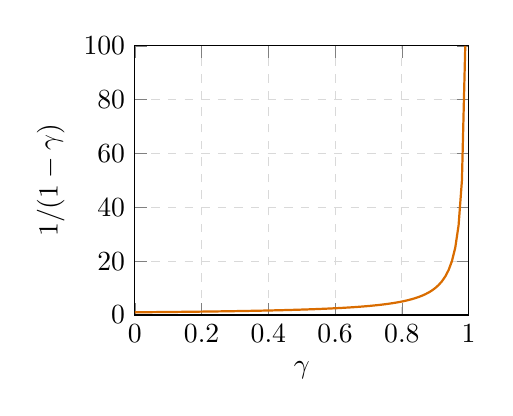
\begin{tikzpicture}
\begin{axis}[width=0.48\linewidth,height=5cm,xlabel={$\gamma$},ylabel={$1/(1-\gamma)$},xmin=0,xmax=1,ymin=0,ymax=100,
  domain=0:0.99,samples=100,grid=both,grid style={dashed,gray!30}]
 \addplot[orange!85!black,thick]{1/(1-x)};
\end{axis}
\end{tikzpicture}
\caption{Left: discount weights $\gamma^h$. Right: the effective horizon $1/(1-\gamma)$ diverges as $\gamma\to1$ (original figures for slide 32).}
\end{figure}

\begin{intuition}
With $\gamma=0.99$ the weight $\gamma^{h}$ falls to $\gamma^{100}\approx0.37\approx1/e$ after about $100$ steps; with $\gamma=0.9$ the same happens after about $10$ steps. If rewards are at most $\Rmax=1$, the value can never exceed $1/(1-0.99)=100$; at $\gamma=1$ the bound is infinite and the sum of rewards of an endless task need not exist at all. The discount is what makes ``the value of a state'' a well-defined finite number.
\end{intuition}

%=====================================================================
\section{Bellman Equation \slr{33--36}}
%=====================================================================
The value of a state is expanded in terms of the current reward and the value of the next states according to the policy (slide 33): for a deterministic $\pi$,
\[
  V^\pi(s_t)=\E_\pi\!\left[r_t+\gamma r_{t+1}+\gamma^2r_{t+2}+\cdots\mid s_t\right]=r_t+\gamma\,\E_{s'\sim p(\cdot\mid s_t,\pi(s_t))}\!\left[V^\pi(s')\right],
\]
and likewise for $Q$ (slides 34--36):
\[
  Q^\pi(s_t,a_t)=r_t+\gamma\,\E_{s'\sim p(\cdot\mid s_t,a_t)}\!\left[V^\pi(s')\right].
\]
In the first equation $r$ is a function of $s$ and $\pi(s)$; in the second, of $s$ and $a$. As a result $V^\pi(s)=Q^\pi(s,\pi(s))$ (slide 36).

\begin{theorem}[Bellman expectation equations]\label{thm:bellexp}
For every policy $\pi$ and all $s,a$:
\begin{align*}
 V^\pi(s)&=\E_{a\sim\pi(\cdot\mid s)}\Big[r(s,a)+\gamma\,\E_{s'\sim p(\cdot\mid s,a)}\big[V^\pi(s')\big]\Big],\\
 Q^\pi(s,a)&=r(s,a)+\gamma\,\E_{s'\sim p(\cdot\mid s,a)}\big[V^\pi(s')\big],\\
 V^\pi(s)&=\E_{a\sim\pi(\cdot\mid s)}\big[Q^\pi(s,a)\big].
\end{align*}
For a deterministic policy the first reads $V^\pi(s)=r(s,\pi(s))+\gamma\E_{s'\sim p(\cdot\mid s,\pi(s))}[V^\pi(s')]$ and the last $V^\pi(s)=Q^\pi(s,\pi(s))$.
\end{theorem}
\begin{proof}
Split the return after the first step using $G_0=r(s_0,a_0)+\gamma G_1$:
$V^\pi(s)=\E^\pi[G_0\mid s_0=s]=\E^\pi[r(s_0,a_0)\mid s_0=s]+\gamma\E^\pi[G_1\mid s_0=s]$.
Condition the second term on $(a_0,s_1)$ and use the tower rule. By Definition~\ref{def:markov} and the fact that $\pi$ depends only on the current state, the conditional distribution of the trajectory from $s_1$ onwards given $(s_0,a_0,s_1)$ is the same as that of a trajectory started at $s_1$; hence $\E^\pi[G_1\mid s_0=s,a_0=a,s_1=s']=V^\pi(s')$. Averaging over $s'\sim p(\cdot\mid s,a)$ and then over $a\sim\pi(\cdot\mid s)$ gives the first identity; the argument for $Q^\pi$ is the same with $a_0$ fixed.
\end{proof}

\begin{figure}[htbp]
\centering
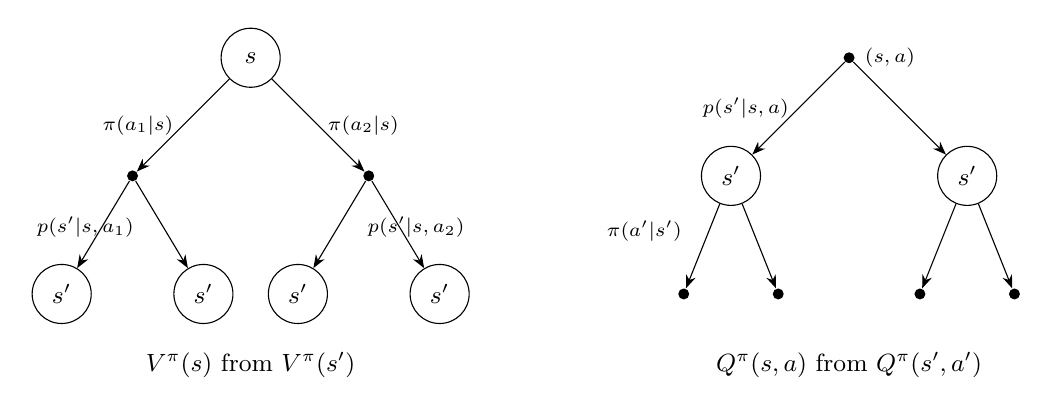
\begin{tikzpicture}[>=Stealth,
  s/.style={circle,draw,minimum size=0.75cm,font=\small},
  a/.style={circle,fill=black,inner sep=1.4pt}]
  % V backup
  \begin{scope}
   \node[s](v) at (0,3){$s$};
   \node[a](a1) at (-1.5,1.5){};\node[a](a2) at (1.5,1.5){};
   \draw[->](v)--(a1) node[pos=0.5,left,font=\scriptsize]{$\pi(a_1|s)$};
   \draw[->](v)--(a2) node[pos=0.5,right,font=\scriptsize]{$\pi(a_2|s)$};
   \node[s](na) at (-2.4,0){$s'$};\node[s](nb) at (-0.6,0){$s'$};
   \node[s](nc) at (0.6,0){$s'$};\node[s](nd) at (2.4,0){$s'$};
   \draw[->](a1)--(na);\draw[->](a1)--(nb);\draw[->](a2)--(nc);\draw[->](a2)--(nd);
   \node[font=\scriptsize] at (-2.1,0.85){$p(s'|s,a_1)$};
   \node[font=\scriptsize] at (2.1,0.85){$p(s'|s,a_2)$};
   \node[font=\small] at (0,-0.9){$V^\pi(s)$ from $V^\pi(s')$};
  \end{scope}
  % Q backup
  \begin{scope}[xshift=7.6cm]
   \node[a,label=right:{\scriptsize $(s,a)$}](q) at (0,3){};
   \node[s](ml) at (-1.5,1.5){$s'$};\node[s](mr) at (1.5,1.5){$s'$};
   \draw[->](q)--(ml) node[pos=0.5,left,font=\scriptsize]{$p(s'|s,a)$};\draw[->](q)--(mr);
   \node[a](b1) at (-2.1,0){};\node[a](b2) at (-0.9,0){};\node[a](b3) at (0.9,0){};\node[a](b4) at (2.1,0){};
   \draw[->](ml)--(b1);\draw[->](ml)--(b2);\draw[->](mr)--(b3);\draw[->](mr)--(b4);
   \node[font=\scriptsize] at (-2.6,0.8){$\pi(a'|s')$};
   \node[font=\small] at (0,-0.9){$Q^\pi(s,a)$ from $Q^\pi(s',a')$};
  \end{scope}
\end{tikzpicture}
\caption{Backup diagrams for the Bellman expectation equations (original figure for slides 33--36).}
\end{figure}

\begin{intuition}
The equation says: \emph{value now = reward now + discounted value of where I land}. It turns an infinite sum into a one-step consistency condition. Example (deterministic): if $r(s,\pi(s))=1$, $\gamma=0.9$ and the next state always has value $V^\pi(s')=10$, then $V^\pi(s)=1+0.9\cdot10=10$. The two lines of the theorem differ only in what is averaged: $V$ averages over my action choice (policy), $Q$ has the first action already fixed and averages only over the environment's randomness.
\end{intuition}

%=====================================================================
\section{Discounted State-Action Distribution \slr{37--38}}
%=====================================================================
\begin{definition}[Discounted state-action distribution]\label{def:dsa}
\[
  d^\pi_{s_0}(s,a)=(1-\gamma)\sum_{h=0}^{\infty}\gamma^h\,\PP^\pi_h(s,a;s_0).
\]
For an initial distribution $\mu$ write $d^\pi_\mu(s,a)=\E_{s_0\sim\mu}[d^\pi_{s_0}(s,a)]$.
\end{definition}

\begin{lemma}[It is a distribution, and that is the point of the $(1-\gamma)$]\label{lem:dist}
$d^\pi_{s_0}$ is a probability distribution over $\cS\times\cA$.
\end{lemma}
\begin{proof}
Non-negativity is clear. Summing over $(s,a)$ and exchanging the (absolutely convergent) sums,
$\sum_{s,a}d^\pi_{s_0}(s,a)=(1-\gamma)\sum_h\gamma^h\sum_{s,a}\PP^\pi_h(s,a;s_0)=(1-\gamma)\sum_h\gamma^h=1$, since $\PP^\pi_h(\cdot;s_0)$ is a distribution for each $h$.
\end{proof}
This matches the slide's remark: ``this gives us a probability distribution (remember $\sum_h\gamma^h=1/(1-\gamma)$)''. The companion identity expressing discounted sums as expectations under $d^\pi_{s_0}$ is not on the slides and is given in Appendix~\ref{app:identity}.

\begin{intuition}
Take the visitation probabilities of the previous section, weight time step $h$ by $\gamma^h$ and sum them: this is ``how much total (discounted) time I spend in $(s,a)$''. Without the factor $(1-\gamma)$ the total mass would be $1/(1-\gamma)$ (e.g.\ $100$ for $\gamma=0.99$); multiplying by $(1-\gamma)$ rescales it to $1$ so it can be used as a genuine probability distribution. Early time steps get most of the weight, which is the same patience dial as before.
\end{intuition}

%=====================================================================
\section{Optimal Policy \slr{39--40}}
%=====================================================================
\begin{definition}[Optimal value and optimal policy]\label{def:opt}
$V^\star(s)=\sup_\pi V^\pi(s)$ and $Q^\star(s,a)=\sup_\pi Q^\pi(s,a)$. A policy $\pi^\star$ is optimal if $V^{\pi^\star}(s)=V^\star(s)$ for every $s$.
\end{definition}

Slides 39--40 state that for infinite-horizon MDPs there \emph{always} exists a deterministic policy $\pi^\star$ such that
\[
  V^{\pi^\star}(s)\ge V^\pi(s)\qquad\forall s,\pi,
\]
i.e.\ $\pi^\star$ dominates all other policies in each state; it returns optimal actions $a^\star$, and $V^{\pi^\star}=V^\star$, $Q^{\pi^\star}=Q^\star$. The existence statement is proved constructively by Theorem~\ref{thm:greedy} below.

\begin{intuition}
It is far from obvious that one policy can be best \emph{in all states simultaneously}; in many optimisation problems the best choice for one objective hurts another. Here it is true, and it is also true that we never need randomness: a table of ``best action in each state'' suffices. This is what makes the search for optimal behaviour tractable.
\end{intuition}

%=====================================================================
\section{Bellman Optimality \slr{41--42}}
%=====================================================================
\begin{theorem}[Bellman optimality equation]\label{thm:bellopt}
\begin{align*}
 V^\star(s)&=\max_a\Big[r(s,a)+\gamma\,\E_{s'\sim p(\cdot\mid s,a)}V^\star(s')\Big],\\
 Q^\star(s,a)&=r(s,a)+\gamma\,\E_{s'\sim p(\cdot\mid s,a)}\Big[\max_{a'}Q^\star(s',a')\Big].
\end{align*}
\end{theorem}
On slide 42 the bracket $r(s,a)+\gamma\E_{s'}V^\star(s')$ is annotated as $Q^\star(s,a)$, so that $V^\star(s)=\max_aQ^\star(s,a)$.

\begin{intuition}
The Bellman \emph{expectation} equation averages over the policy's action; the Bellman \emph{optimality} equation replaces that average by a $\max$: the optimal agent simply takes the best action. All the difficulty of looking arbitrarily far into the future is hidden in $V^\star(s')$: if I knew the optimal value of every neighbour, choosing the best action would be a one-step problem.
\end{intuition}

%=====================================================================
\section{Bellman Optimality Example \slr{43--45}}
%=====================================================================
Assume we know $V^\star$ at $s'$ and $s''$, the two successors of $s$ reached by actions $a'$ and $a''$ (slide 43). Try $a'$, get $r(s,a')$ and compute $Q^\star(s,a')=r(s,a')+\gamma V^\star(s')$; try $a''$ and compute $Q^\star(s,a'')=r(s,a'')+\gamma V^\star(s'')$ (slide 44). Then (slide 45)
\[
  V^\star(s)=\max_{a',a''}\{Q^\star(s,a'),\,Q^\star(s,a'')\}.
\]

\begin{figure}[htbp]
\centering
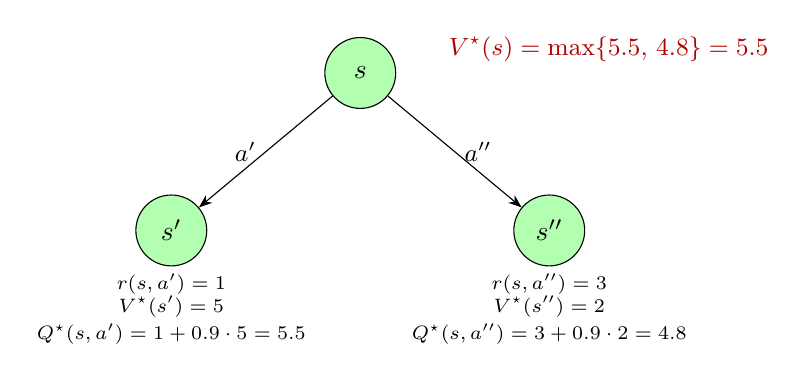
\begin{tikzpicture}[>=Stealth,
  n/.style={circle,draw,fill=green!30,minimum size=0.9cm}]
  \node[n](s) at (0,2){$s$};
  \node[n](s1) at (-2.4,0){$s'$};
  \node[n](s2) at (2.4,0){$s''$};
  \draw[->](s)--(s1) node[midway,left,font=\small]{$a'$};
  \draw[->](s)--(s2) node[midway,right,font=\small]{$a''$};
  \node[font=\scriptsize,align=center] at (-2.4,-1.0){$r(s,a')=1$\\$V^\star(s')=5$\\[2pt]$Q^\star(s,a')=1+0.9\cdot5=5.5$};
  \node[font=\scriptsize,align=center] at (2.4,-1.0){$r(s,a'')=3$\\$V^\star(s'')=2$\\[2pt]$Q^\star(s,a'')=3+0.9\cdot2=4.8$};
  \node[red!70!black,font=\small,anchor=west] at (1.0,2.3){$V^\star(s)=\max\{5.5,\,4.8\}=5.5$};
\end{tikzpicture}
\caption{The one-step lookahead of slides 43--45 with illustrative numbers ($\gamma=0.9$; the numbers are mine, not the slide's).}
\end{figure}

\begin{intuition}
With the numbers above the action with the \emph{larger immediate reward} ($a''$, reward $3$) is \emph{not} the best: $a'$ leads to a state worth $5$, and $1+4.5>3+1.8$. This is the one-step trick that everything else in the course rests on: evaluate each action as ``reward + discounted value of where it leads'' and take the best.
\end{intuition}

%=====================================================================
\section{Bellman Optimality (Theorem 1) \slr{46--49}}
%=====================================================================
\begin{theorem}[Theorem 1 --- greedy with respect to $Q^\star$ is optimal]\label{thm:greedy}
Let $\hat\pi(s)\in\argmax_aQ^\star(s,a)$. Then $V^{\hat\pi}=V^\star$, and therefore $\pi^\star=\hat\pi$ is an optimal policy.
\end{theorem}

\subsection*{Proof as shown on the slides (slides 46--48)}
Starting from $V^\star(s)=\max_a[r(s,a)+\gamma\E_{s'}V^\star(s')]$ and unrolling the equation along $\hat\pi$:
\begin{align*}
V^\star(s)&=r(s,\pi^\star(s))+\gamma\E_{s'}V^\star(s')\\
&\le\max_a\Big[r(s,a)+\gamma\E_{s'}V^\star(s')\Big]=r(s,\hat\pi(s))+\gamma\E_{s'}V^\star(s')\\
&\le r(s,\hat\pi(s))+\gamma\E_{s'\sim p(\cdot|s,\hat\pi(s))}\Big[r(s',\hat\pi(s'))+\gamma\E_{s''}V^\star(s'')\Big]\\
&\le\cdots\le\E\Big[r(s,\hat\pi(s))+\gamma r(s',\hat\pi(s'))+\cdots\Big]=V^{\hat\pi}(s),
\end{align*}
so $V^{\hat\pi}\ge V^\star$ (the leftover term $\gamma^k\E V^\star(s_k)\to0$ since $V^\star$ is bounded, Lemma~\ref{lem:bound}); and $V^\star\ge V^{\hat\pi}$ holds by definition of $V^\star$ as a supremum. Hence $V^{\hat\pi}=V^\star$ and, by slide 49, $\pi^\star=\argmax_aQ^\star(s,a)$ is an optimal policy.

\subsection*{Proof in the companion text (fixed-point argument)}
\begin{proof}
By Theorem~\ref{thm:bellopt}, $V^\star=\mathcal BV^\star$ and $Q^\star(s,a)=r(s,a)+\gamma\E_{s'}[V^\star(s')]$ (the operators $\mathcal B,\mathcal B^{\hat\pi}$ are recalled in Appendix~\ref{app:ops}). Since $\hat\pi(s)$ maximises $Q^\star(s,\cdot)$,
\[
(\mathcal BV^\star)(s)=\max_aQ^\star(s,a)=Q^\star\big(s,\hat\pi(s)\big)=r\big(s,\hat\pi(s)\big)+\gamma\E_{s'\sim p(\cdot|s,\hat\pi(s))}\big[V^\star(s')\big]=(\mathcal B^{\hat\pi}V^\star)(s),
\]
so $V^\star$ is a fixed point of $\mathcal B^{\hat\pi}$. By Theorem~\ref{thm:bellexp} so is $V^{\hat\pi}$, and both are bounded by Lemma~\ref{lem:bound}.

A bounded fixed point of $\mathcal B^{\hat\pi}$ is unique. If $u$ and $v$ are two, then for every $s$
\[
|u(s)-v(s)|=\gamma\Big|\E_{s'}\big[u(s')-v(s')\big]\Big|\le\gamma\|u-v\|_\infty,
\]
because the rewards cancel, so $\|u-v\|_\infty\le\gamma\|u-v\|_\infty$. The norm is finite and $\gamma<1$, hence $u=v$. Therefore $V^{\hat\pi}=V^\star$, and $\hat\pi$ attains the supremum of Definition~\ref{def:opt} at every state.
\end{proof}

\begin{intuition}
Theorem~1 is the license to \emph{act}: once someone hands me $Q^\star$, I do not need to plan any more; the single-step rule ``pick the action with the largest $Q^\star(s,\cdot)$'' is already globally optimal. The slide proof says it as a sandwich: following $\hat\pi$ can't be better than optimal ($V^{\hat\pi}\le V^\star$), and by unrolling the optimality equation it can't be worse either ($V^{\hat\pi}\ge V^\star$). The book proof says the same thing differently: $V^\star$ and $V^{\hat\pi}$ solve the same one-policy equation, and that equation has only one bounded solution because each application shrinks distances by $\gamma<1$.
\end{intuition}

%=====================================================================
\section{Bellman Optimality (Theorem 2) \slr{50--55}}
%=====================================================================
\begin{theorem}[Theorem 2 --- the optimality equation has one solution]\label{thm:unique}
If $V:\cS\to\mathbb R$ satisfies $V(s)=\max_a\big[r(s,a)+\gamma\E_{s'\sim p(\cdot|s,a)}V(s')\big]$ for every $s$, then $V=V^\star$.
\end{theorem}
The slides (51--53) ask us to check that $\|V-V^\star\|_\infty=0$ and then unroll the difference.
\begin{proof}
Both $V$ and $V^\star$ satisfy the same equation, so for every $s$,
\begin{align*}
|V(s)-V^\star(s)|&=\Big|\max_a\big[r(s,a)+\gamma\E_{s'}V(s')\big]-\max_a\big[r(s,a)+\gamma\E_{s'}V^\star(s')\big]\Big|\\
&\le\max_a\Big|\big[r(s,a)+\gamma\E_{s'}V(s')\big]-\big[r(s,a)+\gamma\E_{s'}V^\star(s')\big]\Big|\\
&=\max_a\gamma\Big|\E_{s'\sim p(\cdot|s,a)}\big[V(s')-V^\star(s')\big]\Big|\\
&\le\gamma\max_a\E_{s'\sim p(\cdot|s,a)}\big|V(s')-V^\star(s')\big|.
\end{align*}
The first inequality is $|\max_af(a)-\max_ag(a)|\le\max_a|f(a)-g(a)|$; the last is Jensen. Applying the same bound to $|V(s')-V^\star(s')|$ and iterating $k$ times,
\[
|V(s)-V^\star(s)|\le\gamma^k\max_{a_0,\dots,a_{k-1}}\E_{s_k}\big|V(s_k)-V^\star(s_k)\big|\le\gamma^k\|V-V^\star\|_\infty,
\]
and since $\gamma<1$ and $\|V-V^\star\|_\infty$ is finite, the right-hand side tends to $0$. Hence $|V(s)-V^\star(s)|=0$ for every $s$.
\end{proof}

Slide 54 illustrates the shrinking bound $\gamma^h\|V-V^\star\|_\infty$ as the number of future steps $h$ grows (its example uses $\gamma=0.92$ and a baseline $\|V-V^\star\|_\infty=1$).

\begin{figure}[htbp]
\centering
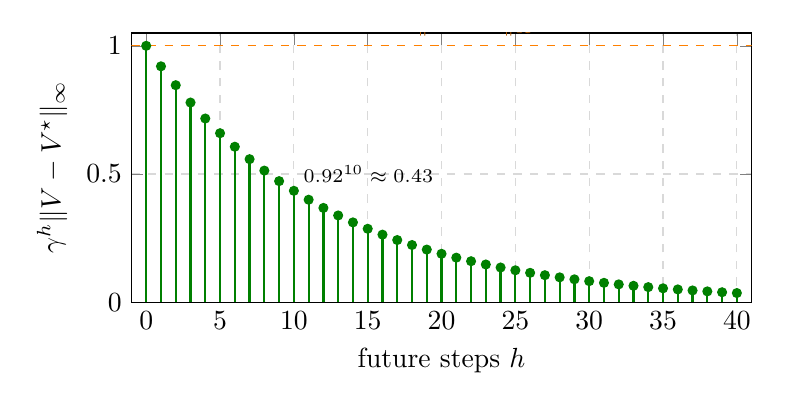
\begin{tikzpicture}
\begin{axis}[width=0.78\linewidth,height=5cm,xlabel={future steps $h$},ylabel={$\gamma^h\|V-V^\star\|_\infty$},
  xmin=-1,xmax=41,ymin=0,ymax=1.05,grid=both,grid style={dashed,gray!30}]
 \addplot[ycomb,green!50!black,thick,mark=*,mark size=1.4pt,domain=0:40,samples=41]{0.92^x};
 \draw[dashed,orange] (axis cs:-1,1)--(axis cs:41,1);
 \node[orange!70!black,font=\scriptsize,anchor=south west] at (axis cs:12,1.0){baseline $\|V-V^\star\|_\infty=1$};
 \node[font=\scriptsize,anchor=west] at (axis cs:10,0.5){$0.92^{10}\approx0.43$};
\end{axis}
\end{tikzpicture}
\caption{The bound $\gamma^h\|V-V^\star\|_\infty$ for $\gamma=0.92$, redrawn from the idea of slide 54 (values computed here).}
\end{figure}

\begin{figure}[H]
	\centering
	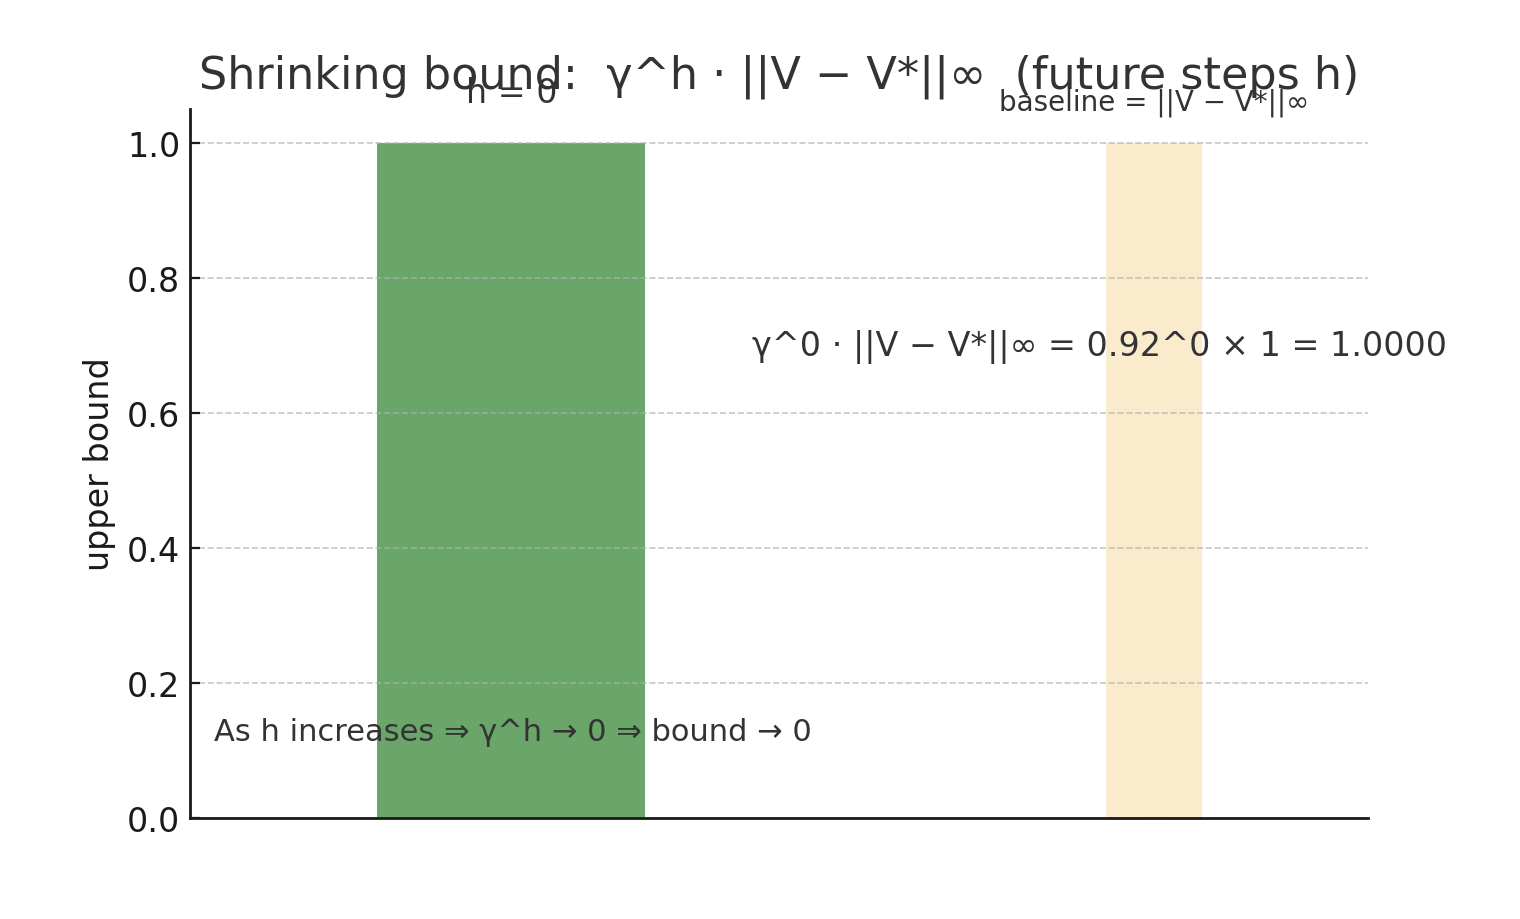
\includegraphics[width=1.0\linewidth]{1790936669032.png}
	\caption{Shrinking bound}\label{fig:1790936669032}
\end{figure}
\begin{intuition}
Imagine a ``fake'' value function $V$ that satisfies the optimality equation and is not $V^\star$. Each time we expand the equation one step, the gap can be at most $\gamma$ times what it was; after $k$ steps it is at most $\gamma^k$ times the original gap, which melts away (with $\gamma=0.92$, $0.92^{56}<0.01$). The only way for the gap to survive all expansions is to be $0$. Slide 55 states the consequence: \emph{we can focus on one step at a time}, leaving the rest of the problem to $V(s')$, and any $V$ satisfying that one-step formula is in fact $V^\star$.
\end{intuition}

%=====================================================================
\section{Summary}
%=====================================================================
\begin{center}
\small
\renewcommand{\arraystretch}{1.35}
\begin{tabular}{@{}>{\raggedright\arraybackslash}p{2.9cm}>{\raggedright\arraybackslash}p{6.3cm}>{\raggedright\arraybackslash}p{4.5cm}c@{}}
\toprule
\textbf{Object / result} & \textbf{Formula} & \textbf{What it tells us} & \textbf{Slides}\\
\midrule
Markov state & $p(s_{t+1}|s_t,a_t)=p(s_{t+1}|h_t,a_t)$ & the present summarises the past & 15--17\\
MDP & $(\cS,\cA,p,r,\gamma)$ & sequential decisions with consequences & 18--29\\
$V^\pi$, $Q^\pi$ & $\E[\sum_h\gamma^hr_{t+h}\mid\cdot]$ & how good a state / action is under $\pi$ & 30--31\\
Finite values & $0\le V^\pi\le\Rmax/(1-\gamma)$ & why $\gamma<1$ & 32\\
Bellman expectation & $V^\pi(s)=\E_a[r+\gamma\E_{s'}V^\pi(s')]$ & one-step consistency of a given policy & 33--36\\
$d^\pi_{s_0}$ & $(1-\gamma)\sum_h\gamma^h\PP^\pi_h$ & discounted occupancy, a true distribution & 37--38\\
Optimal $V^\star,Q^\star$ & $\sup_\pi V^\pi$, $\sup_\pi Q^\pi$ & a deterministic policy dominates all others & 39--40\\
Bellman optimality & $V^\star(s)=\max_a[r+\gamma\E_{s'}V^\star(s')]$ & one-step lookahead with a $\max$ & 41--45\\
Theorem 1 & $\hat\pi\in\argmax_aQ^\star\Rightarrow V^{\hat\pi}=V^\star$ & greedy w.r.t.\ $Q^\star$ is optimal & 46--49\\
Theorem 2 & $V=\max_a[r+\gamma\E V]\Rightarrow V=V^\star$ & $V^\star$ is the unique solution & 50--55\\
\bottomrule
\end{tabular}
\end{center}

\begin{figure}[htbp]
\centering
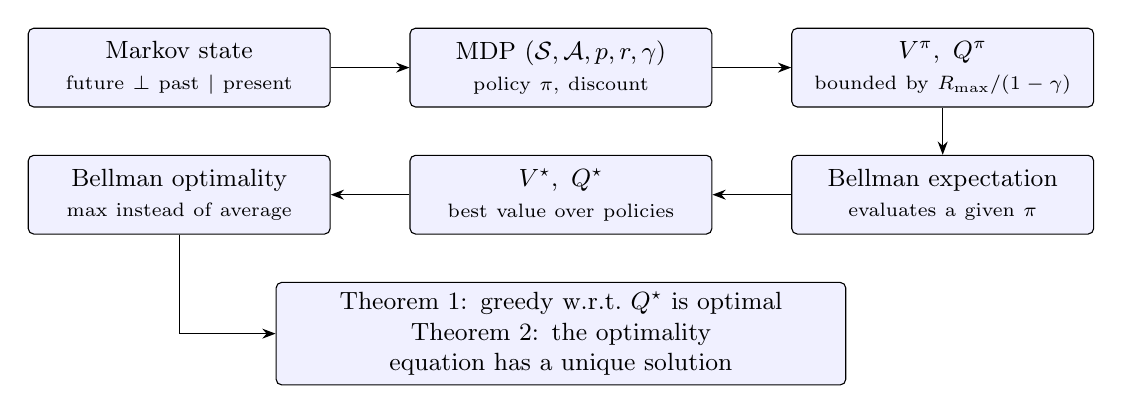
\begin{tikzpicture}[>=Stealth,node distance=6mm and 10mm,
  b/.style={draw,rounded corners=2pt,fill=blue!6,align=center,minimum height=1.0cm,text width=3.6cm,font=\small}]
  \node[b](m){Markov state\\{\scriptsize future $\perp$ past $\mid$ present}};
  \node[b,right=of m](d){MDP $(\cS,\cA,p,r,\gamma)$\\{\scriptsize policy $\pi$, discount}};
  \node[b,right=of d](v){$V^\pi,\ Q^\pi$\\{\scriptsize bounded by $\Rmax/(1-\gamma)$}};
  \node[b,below=of v](be){Bellman expectation\\{\scriptsize evaluates a given $\pi$}};
  \node[b,left=of be](vs){$V^\star,\ Q^\star$\\{\scriptsize best value over policies}};
  \node[b,left=of vs](bo){Bellman optimality\\{\scriptsize $\max$ instead of average}};
  \node[b,below=of vs,text width=7cm](th){Theorem 1: greedy w.r.t.\ $Q^\star$ is optimal\\Theorem 2: the optimality equation has a unique solution};
  \draw[->](m)--(d);\draw[->](d)--(v);\draw[->](v)--(be);\draw[->](be)--(vs);\draw[->](vs)--(bo);\draw[->](bo)|-(th);
\end{tikzpicture}
\caption{Roadmap of the lecture: from the Markov assumption to optimal policies.}
\end{figure}

\subsection*{Key take-aways}
\begin{itemize}
  \item An MDP is a contextual bandit whose next context depends on the action taken; the Markov property means the current state is all the agent needs to know.
  \item The discount factor $\gamma<1$ keeps the value finite, with $0\le V^\pi\le\Rmax/(1-\gamma)$, and $1/(1-\gamma)$ is the effective horizon ($\gamma=0.99\Rightarrow{\sim}100$ steps).
  \item Bellman equations turn an infinite-horizon sum into a one-step relation: value now $=$ reward $+$ discounted value of the next state (average for a policy, $\max$ for optimality).
  \item Theorem 1: acting greedily with respect to $Q^\star$ is optimal, so a deterministic stationary policy always suffices.
  \item Theorem 2: $V^\star$ is the \emph{only} solution of the Bellman optimality equation, thanks to the $\gamma$-contraction; any $V$ that satisfies the one-step formula is $V^\star$.
\end{itemize}

%=====================================================================
\appendix
\section{Appendix: supplementary material (in the companion PDF, not on the slides)}
%=====================================================================
The following results appear in the companion PDF but have no corresponding slide; they are \emph{not} part of the slide flow above.

\subsection{Discounted sums as expectations under \texorpdfstring{$d^\pi_{s_0}$}{d}}\label{app:identity}
\begin{lemma}[Second part of Lemma 5 of the PDF]
For every bounded $f$,
\[
  \E^\pi\!\left[\sum_{h=0}^\infty\gamma^hf(s_h,a_h)\;\Big|\;s_0\right]=\frac1{1-\gamma}\,\E_{(s,a)\sim d^\pi_{s_0}}\big[f(s,a)\big].
\]
\end{lemma}
\begin{proof}
It is the same exchange of (absolutely convergent) sums used in the proof of Lemma~\ref{lem:dist}, applied to $f$: $\E^\pi[\sum_h\gamma^hf(s_h,a_h)\mid s_0]=\sum_h\gamma^h\sum_{s,a}\PP^\pi_h(s,a;s_0)f(s,a)=\frac1{1-\gamma}\sum_{s,a}d^\pi_{s_0}(s,a)f(s,a)$.
\end{proof}
\begin{intuition}
Choosing $f=r$ gives $V^\pi(s_0)=\frac1{1-\gamma}\E_{(s,a)\sim d^\pi_{s_0}}[r(s,a)]$: the value is the average reward under the discounted occupancy, scaled by the effective horizon $1/(1-\gamma)$. For $\gamma=0.9$, if the average reward under $d^\pi$ is $0.5$, the value is $0.5/0.1=5$.
\end{intuition}

\subsection{Bellman operators (notation used in the PDF's proofs)}\label{app:ops}
The proof of Theorem~\ref{thm:greedy} in the companion text uses two operators acting on bounded functions $V:\cS\to\mathbb R$:
\begin{align*}
  (\mathcal BV)(s)&=\max_a\Big[r(s,a)+\gamma\E_{s'\sim p(\cdot|s,a)}V(s')\Big],\\
  (\mathcal B^{\pi}V)(s)&=r(s,\pi(s))+\gamma\E_{s'\sim p(\cdot|s,\pi(s))}V(s')\quad(\pi\text{ deterministic}).
\end{align*}
With this notation Theorem~\ref{thm:bellopt} reads $V^\star=\mathcal BV^\star$, Theorem~\ref{thm:bellexp} reads $V^\pi=\mathcal B^\pi V^\pi$, and Theorem~\ref{thm:unique} says that $\mathcal B$ has a unique fixed point. The slides never name these operators.

\end{document}